% !TeX program = lualatex

\documentclass{../awesomecv}

\newcommand{\name}{Nikos Tsiknakis}

\usepackage{geometry}
\geometry{
  left     =  20mm,
  right    =  20mm,
  bottom   =  23mm,
  top      =  10mm,
  footskip =  10mm
}

\usepackage{fancyhdr}
\pagestyle{fancy}
\fancyhf{}
\renewcommand{\headrulewidth}{0pt}
\lfoot{{\footnotesize\color{\secondfont}\today}}
\cfoot{{\footnotesize\color{\secondfont}\name}}
\rfoot{{\footnotesize\color{\secondfont}\thepage}}

\documentcolor{blue}
\secondcolor{base01}
\thirdcolor{base01}
\sectioncolor{base02}

\titlethicknessleft{3mm}

\voiceleftsize{2.1cm}
\voicerightsize{12cm}

\begin{document}

% \pagenumbering{gobble}

\begin{titlebox}
  \authorname{Nikos Tsiknakis}{\emph{Curriculum Vit\ae}}

  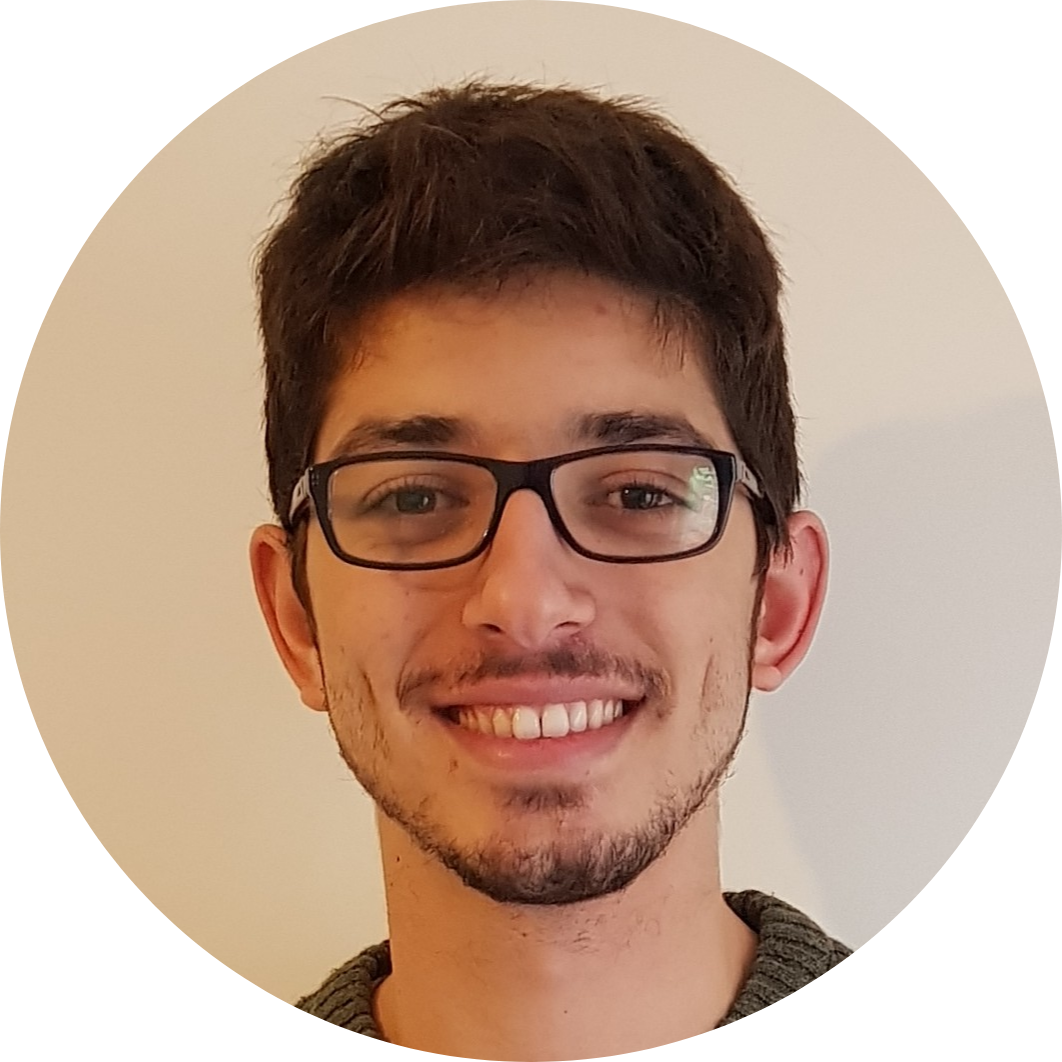
\includegraphics[scale=0.1]{images/tsiknakis.png}
  % \qrcode{../pics/qrcode.png}

  \tcblower

  \begin{showinfo}
    \birthdate{$17^{\text{th}}$ April, 1996}
    \location{Heraklion, Greece}
    \phone{+30 6947478728}
    \firstMail{\href{mailto:tsiknakisn@gmail.com}{tsiknakisn@gmail.com}}
    \otherMail{\href{mailto:tsiknakisn@ics.forth.gr}{tsiknakisn@ics.forth.gr}}
    \github{ \href{https://github.com/tsikup}{tsikup} }
    % \twitter{https://twitter.com/BryanCranston}
    \generic{\faLinkedin}{ \href{https://www.linkedin.com/in/tsiknakisn/}{tsiknakisn} }
    \generic{\faFirefox}{ \href{https://tsikup.github.io}{tsikup.github.io} }
  \end{showinfo}

\end{titlebox}

\updated{}
% \vspace{20pt}

% ********************* %
% *     EDUCATION     * %
% ********************* %
\opensection{\faBook}{Education}
\begin{describesection}

  \leftside{\bf Sep 2014 - Jul 2019}
  \rightsidecomplex{BEng - MEng in Electrical and Computer Engineering}{University of Patras}{}{5 years Integrated Masters 300 ECTS degree - Graduated 3rd in my class with a grade of 8.3/10}

  \leftside{Thesis}
  \rightsideplain{\textsc{Stereo Vision of Dual View Meteosat Images} \href{https://tsikup.github.io/assets/pdf/tsik-thesis.pdf}{(\textcolor{blue}{link})}}
  \leftside{Supervisor}
  \rightsideplain{\href{http://www.ece.upatras.gr/skodras/}{Prof. Athanassios Skodras} \vspace{6pt}}

  \leftside{\bf 2010 - 2014}
  \rightsidecomplex{Secondary Education}{2nd High School}{Heraklion, Greece}{Graduated with hounors and a grade of 19.0/20.0}

  \leftside{}
  \rightsideplain{In 2014 I participated at the National University Entrance Exams in which I obtained a GPA: 18.753/20.000}

\end{describesection}

% ********************* %
% *     EXPERIENCE    * %
% ********************* %
\opensection{\faBlackTie}{Experience}
\begin{describesection}

  % WORK 1
  \leftside{\bf Sep 2019 - }
  \rightsidecomplex{Software Engineer}{Computational Biomedicine Laboratory ICS FORTH}{Heraklion, Greece}{}

  % Intership
  \leftside{\bf Jul 2018 - Sep 2018}
  \rightsidecomplex{Intern}{Computational Biomedicine Laboratory ICS FORTH}{Heraklion, Greece}{}

  % \subdescription{base01}{\faTrophy}{Products}

  % \leftside{name}
  % \rightsideplain{\color{blue}Blue Sky}

  % \leftside{description}
  % \rightsideplain{\emph{Blue Sky is the bomb, bitch. Have you ever seen a
  %     quality of 99.1\%?}}

\end{describesection}

% ********************* %
% *      SEMINARS     * %
% ********************* %
\opensection{\faFlask}{Seminars \& Workshops}
\begin{describesection}

  \leftside{\bf 28-31 Aug 2018}
  \rightsidecomplex{Drone School \& Workshops: Deep learning and Computer vision for drone imaging and cinematography}{Icarus Group CSD AUTH}{}{\url{http://icarus.csd.auth.gr/activities/droneschool/} \vspace{5pt}}

  \leftside{}
  \rightsideplain{I remotely attented the summer school which provided an in depth overview of the various computer vision and deep learning problems encountered in drone imaging and cinematography and corresponding applicable methods. \vspace{15pt}}

  \leftside{\bf 12-14 Feb 2018}
  \rightsidecomplex{MEDDAYS 2018}{Sophia Antipolis}{}{\url{http://leat.unice.fr/MEDDAYS2018/\#page=home} \vspace{5pt}}

  \leftside{}
  \rightsideplain{I was selected to be one of 35 University students in total from Greece, Italy, Spain, Algeria, Morocco, Tunisia, Lebanon, Egypt and Turkey, to attend the fifth edition of the «Mediterranean Days@Campus SophiaTech» event. The goal was to present to selected students, the Sophia Antipolis campus, the research activities of selected highly visible laboratories with a focus on offered international master and doctoral studies. \vspace{15pt}}

  \leftside{\bf 18-20 Oct 2017}
  \rightsidecomplex{Autumn School Aeroworks}{University of Patras}{}{\url{http://www.aeroworks2020.eu/school} \vspace{5pt}}

  \leftside{}
  \rightsideplain{The above summer school focused on providing insights and high tech knowledge on Aerial Robotics and specifically in the following domains: (a) Aerial manipulation, (b) Vision for aerial manipulation, (c) Cooperative aerial coverage, (d) Modeling and Control of UAVs, (e) Estimation and Sensor fusion for UAVs, (f) Aerial reconstruction and inspection. \vspace{15pt}}

  \leftside{\bf 10-15 Jul 2016}
  \rightsidecomplex{1st Interdisciplinary Summer School on Privacy (ISP 2016)}{Nijmegen, Netherlands}{}{\url{https://isp.cs.ru.nl/2016/} \vspace{5pt}}

  \leftside{}
  \rightsideplain{The interdisciplinary summer school on privacy provided an intensive one week academic postgraduate programme teaching privacy from a technical, legal and social perspective. The goal of the summer school was to provide students with a solid background in the theory of privacy construction, modelling and protection from these three different perspectives. \vspace{15pt}}

  \leftside{\bf 22-24 Apr 2016}
  \rightsidecomplex{9 th Panhellenic Conference of ECE Students}{Chania, Greece}{}{\url{https://sfhmmy9.sfhmmy.gr/} \vspace{5pt}}

\end{describesection}

% ********************* %
% *       AWARDS      * %
% ********************* %
\opensection{\faDiamond}{Prizes and Awards}
\begin{describesection}

  \leftside{\bf Feb 2014}
  \rightsidecomplex{Best 1st year's project, Introduction to Programming Course}{ECE University of Patras}{}{}

  \leftside{}
  \rightsideplain{I was part of a team (7 members) that was awarded the best 1st year’s project award for the Introduction to Programming Course. We worked with the programming language Python for the design, implementation and testing of an integrated Image Editor and Viewer supporting an interactive graphical user interface.}

\end{describesection}

% *************************** %
% *       PUBLICATIONS      * %
% *************************** %
\opensection{\faBook}{Publications in International Conferences}
\begin{describesection}

  \leftside{1.}
  \rightsideplain{C. Spanakis, E. Mathioudakis, N. Kampanis, N. Tsiknakis, K. Marias, Renyi divergence and non-deterministic subsampling in Rigid Image Registration, 2019 IEEE International Conference on Imaging Systems and Techniques (IST)}

\end{describesection}


% ************************ %
% *     CERTIFICATES     * %
% ************************ %
\opensection{\faCertificate}{Certificates}
\begin{describesection}

  \leftside{\bf Oct 2019}
  \rightsidecomplex{Deep Learning Specialization}{Coursera}{}{\url{https://www.coursera.org/account/accomplishments/specialization/2X3DAMJNRWQ4} \vspace{5pt}}

  \leftside{\bf Oct 2019}
  \rightsidecomplex{Sequence Models}{Coursera}{}{\url{https://www.coursera.org/account/accomplishments/verify/KCLX2DCF9J89} \vspace{5pt}}

  \leftside{\bf Sep 2019}
  \rightsidecomplex{Convolutional Neural Networks}{Coursera}{}{\url{https://www.coursera.org/account/accomplishments/verify/4GRNSJPW5KW9} \vspace{5pt}}

  \leftside{\bf Sep 2019}
  \rightsidecomplex{Structuring Machine Learning Projects}{Coursera}{}{\url{https://www.coursera.org/account/accomplishments/verify/EGYB8W3WLY28} \vspace{5pt}}

  \leftside{\bf Sep 2019}
  \rightsidecomplex{Improving Deep Neural Networks: Hyperparameter tuning, Regularization and Optimization}{Coursera}{}{\url{https://www.coursera.org/account/accomplishments/verify/FPQQ6YWKQK7P} \vspace{5pt}}

  \leftside{\bf Sep 2019}
  \rightsidecomplex{Neural Networks and Deep Learning}{Coursera}{}{\url{https://www.coursera.org/account/accomplishments/verify/P7AE9CDMRBEE} \vspace{5pt}}

\end{describesection}

% ********************* %
% *       SKILLS      * %
% ********************* %
\opensection{\faDiamond}{SKILLS}
\begin{describesection}

  \leftside{\bf Programming Skills}
  \rightsidecomplex{Advanced}{C, Python, Java, Matlab, SQL, HTML, CSS, JavaScript}{}{}

  \leftside{}
  \rightsidecomplex{Very Good}{C++}{}{}

  \leftside{}
  \rightsidecomplex{Good}{Prolog}{}{}

  \leftside{\bf Tools, Frameworks \& Technologies}
  \rightsidecomplex{\vspace{-11pt}}{Tensorflow \& Keras Frameworks \newline
  Django, Node.js, SQL (MySQL), NoSQL (MongoDB) \newline
  Unix/Linux OS and Git Version Control \newline
  Texas Instruments DSK6713 Digital Signal Processor \newline
  Microsoft Office \& LaTeX \newline
  Abode Lightroom \newline
  AutoCAD \newline
  }{}{}

\end{describesection}

% ************************ %
% *     UNI PROJECTS     * %
% ************************ %
\opensection{\faBug}{Major University Projects}
\begin{describesection}

  \leftside{\bf Oct 2017 – Feb 2018}
  \rightsidecomplex{IEEE Signal Processing Society SPCup2018}{5 members group - ECE University of Patras}{}{\url{https://piazza.com/ieee_sps/other/spcup2018/home} \vspace{5pt}}

  \leftside{\bf 2014-2019}
  \rightsidecomplex{IEEE Xtreme and IEEE Activities}{ECE University of Patras}{}{}

\end{describesection}


% ********************** %
% *     MEMBERSHIPS    * %
% ********************** %
\opensection{\faGroup}{Memberships}
\begin{describesection}

  \leftside{\bf 2016 - 2019}
  \rightsideplain{IEEE and IEEE Signal Processing Society Student Member}

\end{describesection}

\opensection{\faComments}{Languages}
\begin{describesection}

  \leftside{\color{blue}Greek}
  \rightsideplain{Mother tongue}

  \leftside{\color{blue}English}
  \rightsideplain{Excellent \emph{(C2 Certificate of Proficiency University of Michigan)}}

  \leftside{\color{blue}German}
  \rightsideplain{Good \emph{(B1 Goethe Institute)}}

\end{describesection}

\end{document}
